\documentclass[11pt,oneside]{article}
\usepackage[T1]{fontenc}
\usepackage[utf8]{inputenc}
%\DeclareUnicodeCharacter{00A0}{ }
\usepackage[adobe-utopia]{mathdesign}

\usepackage{amsmath}
\usepackage[francais]{babel}
\usepackage[dvips]{graphicx}
%\usepackage{here}
\usepackage{framed}
\usepackage[normalem]{ulem}
\usepackage{fancyhdr}
\usepackage{titlesec}
\usepackage{vmargin}

\usepackage{amsmath}
\usepackage{ifthen}
\usepackage{multirow}
\usepackage{multicol} % Portions de texte en colonnes

%\usepackage{xltxtra} % Logo XeLaTeX
%\usepackage{pst-solides3d}
\usepackage{color}
%\usepackage{colortbl}
\usepackage{titletoc} % Pour la mise en forme de la table des matières

%\usepackage[crop=off]{auto-pst-pdf}
%\usepackage{bclogo}


%\usepackage{longtable}
%\usepackage{flafter}%floatants après la référence
%\usepackage{pst-solides3d}
%\usepackage{pstricks}
%\usepackage{minitoc}
%\setcounter{minitocdepth}{4}
%\usepackage{draftcopy}% "Brouillon"
%\usepackage{floatflt}
%\usepackage{psfrag}
%\usepackage{listings} % Permet d'insérer du code de programmation
%\usepackage{lmodern}
%\usepackage[adobe-utopia,uppercase=upright,greeklowercase=upright]{mathdesign}
%\usepackage{minionpro}
%\usepackage{pifont}
%\usepackage{amssymb}
%\usepackage[francais]{varioref}

\setmarginsrb{1.5cm}{1cm}{1cm}{1.5cm}{1cm}{1cm}{1cm}{1cm}

\definecolor{gris25}{gray}{0.75}
\definecolor{bleu}{RGB}{18,33,98}
\definecolor{bleuf}{RGB}{42,94,171}
\definecolor{bleuc}{RGB}{231,239,247}
\definecolor{rougef}{RGB}{185,18,27}
\definecolor{rougec}{RGB}{255,230,231}
\definecolor{vertf}{RGB}{103,126,82}
\definecolor{vertc}{RGB}{220,255,191}
\definecolor{violetf}{RGB}{112,48,160}
\definecolor{violetc}{RGB}{230,224,236}
\definecolor{jaunec}{RGB}{220,255,191}

\usepackage{style/schemabloc}
%Si le boolen xp est vrai : compilation pour xabi
%Sinon compilation Damien
\newboolean{xp}
\setboolean{xp}{true}

\newboolean{prof}
\setboolean{prof}{true}

\def\xxtitre{\ifthenelse{\boolean{xp}}{
CI 2 -- SLCI : Étude du comportement des Systèmes Linéaires Continus Invariants}{
}}

\def\xxsoustitre{\ifthenelse{\boolean{xp}}{
Exercice de colle}{
}}


\def\xxauteur{\ifthenelse{\boolean{xp}}{
\noindent 2013 -- 2014 \\
Alain \textsc{Caignot}}{
}}


\def\xxpied{\ifthenelse{\boolean{xp}}{
CI 2 : SLCI\\
Exercice de colle \ifthenelse{\boolean{prof}}{P}{E}%
}{
}}

\usepackage[%
    pdftitle={SLCI - Systèmes du second ordre},
    pdfauthor={Xavier Pessoles},
    colorlinks=true,
    linkcolor=blue,
    citecolor=magenta]{hyperref}



\usepackage{pifont}
\sloppy
\hyphenpenalty 10000


\begin{document}






% \makeatletter \let\ps@plain\ps@empty \makeatother
%% DEBUT DU DOCUMENT
%% =================




%------------- En tetes et Pieds de Pages ------------


\pagestyle{fancy}
\ifthenelse{\boolean{xp}}{%
\renewcommand{\headrulewidth}{0pt}}{%
\renewcommand{\headrulewidth}{0.2pt}} %pour mettre le trait en haut
%\renewcommand{\headrulewidth}{0.2pt}

\fancyhead{}
\fancyhead[L]{%
\ifthenelse{\boolean{xp}}{%
\noindent\begin{minipage}[c]{2.6cm}%

\includegraphics[width=2cm]{png/logo_ptsi.png}%
\end{minipage}%
}{%
\footnotesize{\textit{\textsf{Lycée François Premier}}}
}}

\ifthenelse{\boolean{xp}}{%
\fancyhead[C]{\rule{12cm}{.5pt}}}{
}


\fancyhead[R]{%
\noindent\begin{minipage}[c]{3cm}
\begin{flushright}
\footnotesize{\textit{\textsf{Sciences Industrielles \\ de l'ingénieur}}}%
\end{flushright}
\end{minipage}
}


\ifthenelse{\boolean{xp}}{%
\fancyhead[C]{\rule{12cm}{.5pt}}}{
}

\renewcommand{\footrulewidth}{0.2pt}

\fancyfoot[C]{\footnotesize{\bfseries \thepage}}
\fancyfoot[L]{%
\begin{minipage}[c]{.2\linewidth}
\noindent\footnotesize{{\xxauteur}}
\end{minipage}
\ifthenelse{\boolean{xp}}{}{%
\begin{minipage}[c]{.15\linewidth}

\includegraphics[width=2cm]{png/logoCC.png}
\end{minipage}}
}


\fancyfoot[R]{\footnotesize{\xxpied}}



\begin{center}
 \Large\textsc{\xxtitre}
\end{center}

\begin{center}
 \large\textsc{\xxsoustitre}
\end{center}

%\vspace{.5cm}

\begin{center}
 \large\textsc{Étude du plan horizontal réglable (PHR) de l'airbus A340}
\end{center}

\begin{flushright}
\textit{D'après ressources d'Alain Caignot.}
\end{flushright}



%\begin{center}
%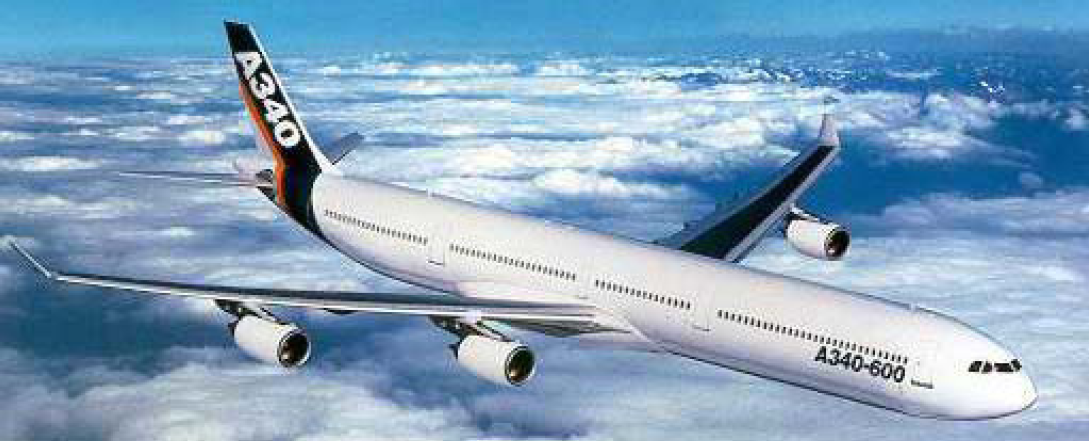
\includegraphics[width=.7\textwidth]{png/image1}
%\end{center}

\section{Présentation}
Le thème proposé concerne l'aéronautique et plus particulièrement la commande en position du plan horizontal réglable (PHR) de l'airbus A340. 

%Gros porteur, très long courrier, ce quadriréacteur symbolise l'aboutissement de la politique de la gamme menée par le conducteur européen depuis le commercialisation de son premier avion, l'A300.
%
%\begin{center}
%\begin{tabular}{ccc}
%\hline
%Spécifications & A340-500 & A340-600 \\
%\hline
%\hline
%Longueur & 67,90 m & 75,30 m \\
%Envergure & 63,45 m & 63,45 m  \\
%Surface ailaire & 437 $m^2$ & 437 $m^2$  \\
%Capacité en sièges & 313 & 378 \\
%Autonomie (km)/Nm & 15.800/8.500 & 13.900/7.500 \\
%Poids au décollage & 368 t & 369 t \\
%Capacité des réservoirs & 214.800 & 194.880 \\
%Moteurs & Trent 553 & Trent 556 \\
%Puissance des moteurs (lbs) & 53.000 & 56.000 \\
%\hline
%\end{tabular}
%\end{center}
%
%\begin{center}
%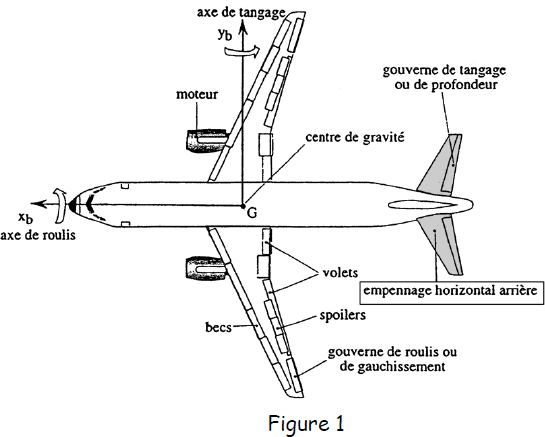
\includegraphics[width=.65\textwidth]{png/image2}
%\end{center}
%
%Le PHR est réglé à l’aide des gouvernes de profondeur (voir Figure 1). On peut montrer que pour une
%vitesse donnée, il est possible, par réglage du PHR, de réduire la poussée des réacteurs et donc
%d’économiser du carburant.
%
%Afin de répondre aux exigences de fiabilité qui stipulent, en particulier, que le PHR doit pouvoir
%fonctionner durant 109 FH (Fly Hour) sans subir de défaillance, un certain nombre de composants de la
%chaîne de commande du PHR sont doublés ou triplés suivant les cas.
%
%D’autre part, toujours par souci de sécurité, le PHR peut être commandé :
%\begin{itemize}
%\item soit automatiquement par un ordinateur de bord qui détermine, à partir des paramètres du vol,
%la valeur optimale de l’angle $\beta$ que doit prendre les gouvernes de profondeur,
%\item soit manuellement par le pilote à partir d’un volant de commande situé dans le poste de pilotage
%et ce en cas de défaillance de la commande automatique du PHR.
%\end{itemize}
%
%La figure 2 présente le schéma de principe de la chaîne d’action à partir de la génération de la
%commande par le calculateur ou le pilote.

Le calculateur génère une tension de commande qui va alimenter le moteur électrique qui est asservi en
position angulaire pour permettre de générer l’angle de consigne initial. Cet angle de consigne initial est
adapté à l’aide du réducteur 1. L’angle de sortie du réducteur 1 permet de commander les deux
distributeurs proportionnels, qui vont délivrer un débit de fluide hydraulique pour alimenter les deux
moteurs hydrauliques. Ces deux moteurs hydrauliques transforment l’énergie hydraulique en énergie
mécanique de rotation. Les deux mouvements de rotation ainsi générer sont additionnés à l’aide du
différentiel pour créer un seul mouvement de rotation à sa sortie. La sortie du différentiel est reliée
au réducteur 6 qui va adapter l’énergie mécanique de puissance pour actionner la vis 4. La vis 4 est
reliée à la gouverne de profondeur et permet de commander son angle.

L’angle de rotation de la vis 4 est capté à l’aide du réducteur 7 qui va l’adapter afin d’être comparé à la
rotation de commande des distributeurs à l’aide du train épicycloïdal, qui joue ici le rôle d’un
comparateur.


%
%\subsection*{Analyse fonctionnelle}
%\subparagraph{Question 1}
%\textit{Compléter le diagramme FAST relatif à la fonction principale régler l’angle du PHR sur le
%document réponse DR1.}
%
%
%\begin{center}
%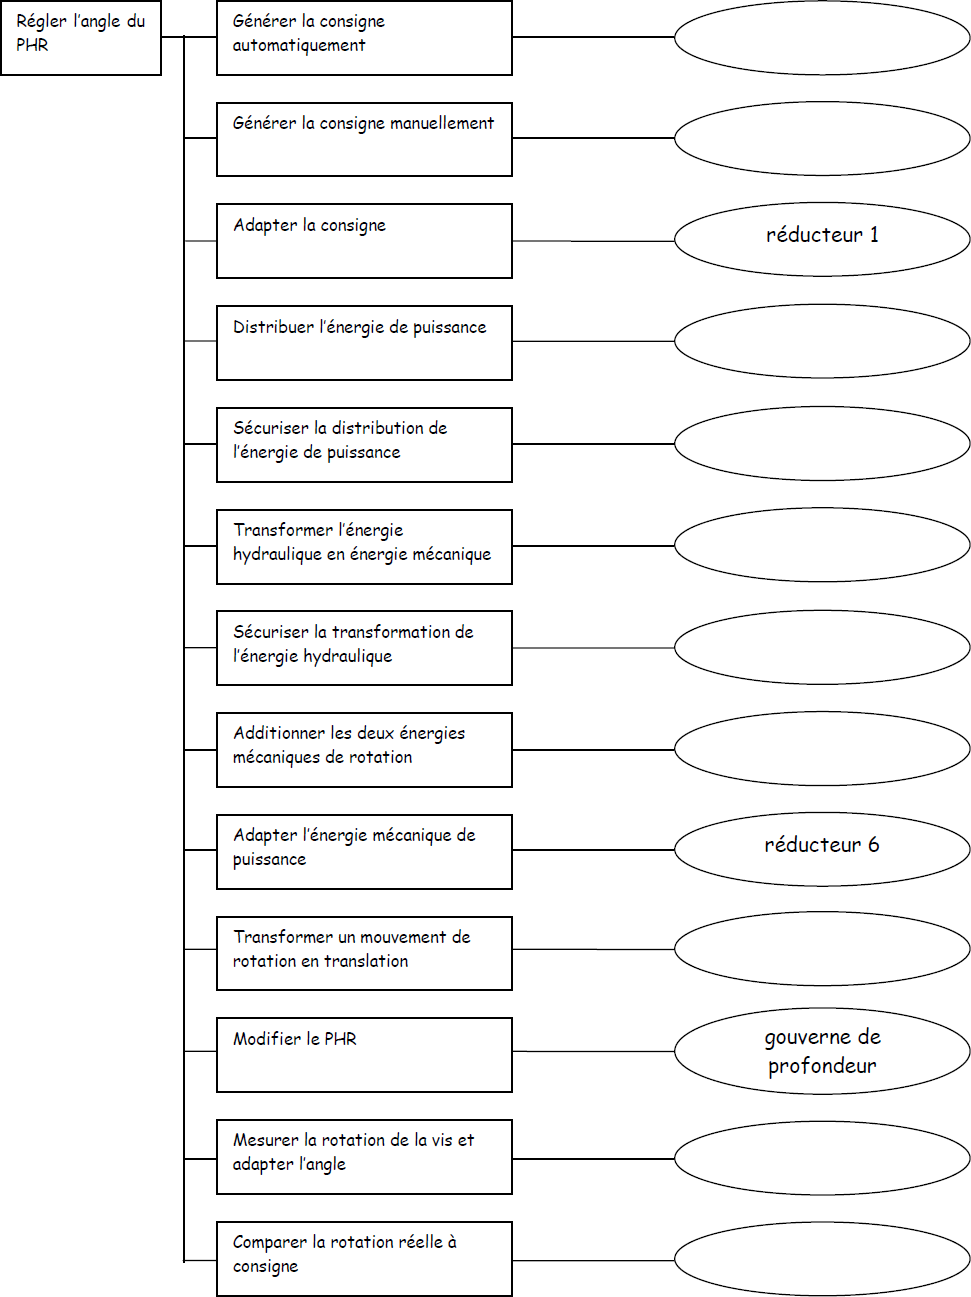
\includegraphics[width=\textwidth]{png/image6}
%\end{center}

\begin{center}
%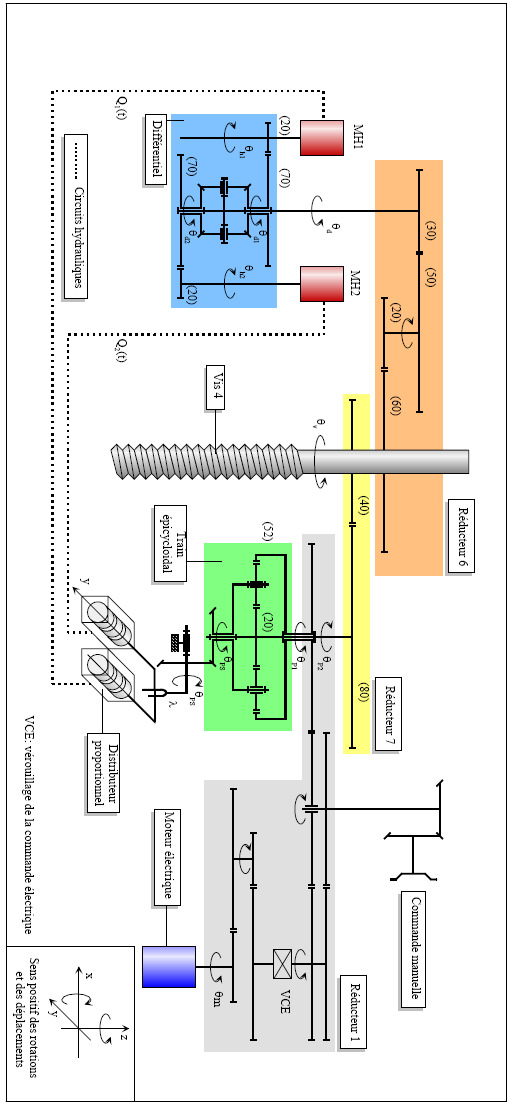
\includegraphics[height=.95\textheight]{png/image3}
\rotatebox{90}{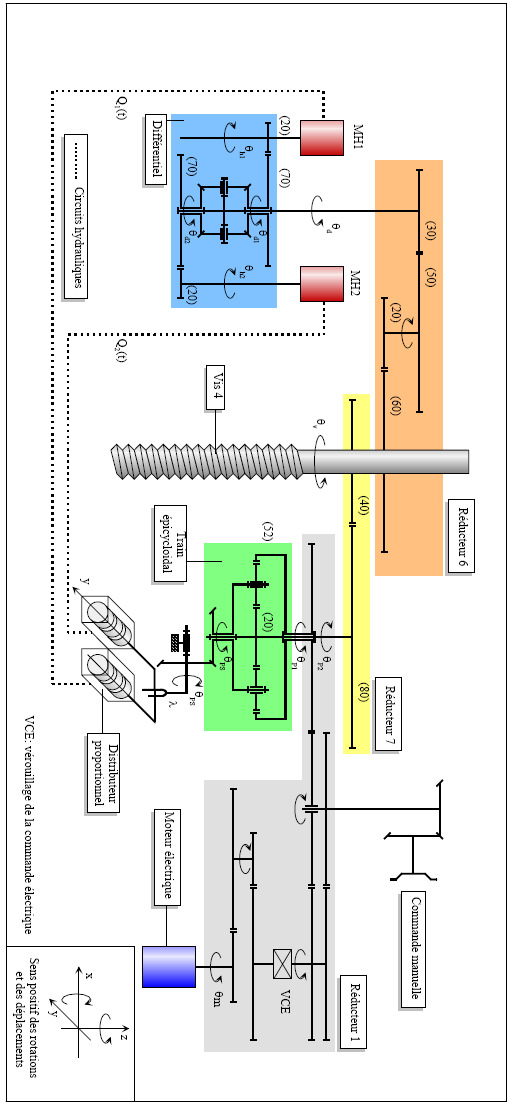
\includegraphics[height=\textwidth]{png/image3}}

Figure 3
\end{center}

\section{\'Etude de l'asservissement en position du moteur électrique}
%
%On se propose d'étudier précisément la boucle d'asservissement en position angulaire du moteur électrique. L'entrée de cet asservissement est une tension de consigne $U_e$ générée par le calculateur. Cette tension est comparée à une tension $U_r$, image de l'angle $\theta_r$, délivrée par un capteur potentiométrique. L'écart $\varepsilon_1$ est ensuite corrigé et amplifié par un bloc correcteur et amplificateur et fournit la tension $U$ aux bornes du moteur électrique. L'angle de rotation $\theta_m$ en sortie du moteur est réduit par un réducteur \textbf{2} pour donner la rotation $\theta_r$ mesurée par le capteur. D'autre part, l'angle $\theta_m$ est réduit par un réducteur \textbf{1} pour fournir un angle de rotation en sortie $\theta_{P1}$, sortie de cet asservissement. 
%
%\subparagraph{Question 2}
%\textit{Construire le schéma bloc fonctionnel de cet asservissement.}

\subsection{Analyse du moteur électrique}
Le moteur électrique est un moteur à courant continu. Les ingénieurs procèdent à une identification du
moteur en le soumettant à un échelon de tension $U=5V$, afin de déterminer par un modèle de
comportement sa fonction de transfert. On obtient la réponse indicielle (vitesse de rotation $\omega_m(t)$ )
donnée ci-après.

\subparagraph{}
\textit{Identifier la réponse en justifiant le modèle retenu et la (ou les) techniques utilisées pour
déterminer les paramètres. Les tracés seront laissés apparents sur la figure ci-après.}


\begin{center}
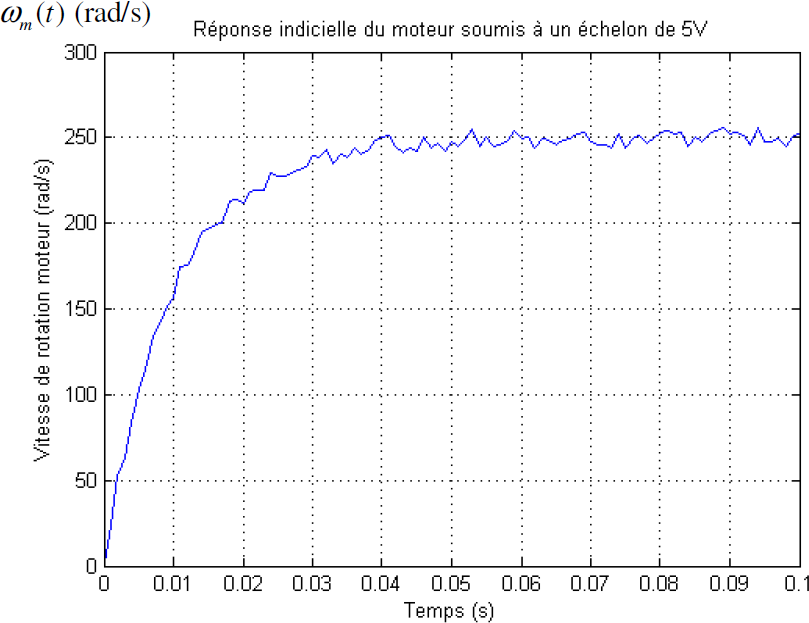
\includegraphics[width=.8\textwidth]{png/image7}
\end{center}


Pour valider le modèle expérimental, on peut utiliser les équations du moteur à courant continu :
\begin{itemize}
\item équation électrique liant la tension $u$ aux bornes du moteur et le courant $i$ le traversant :
$u(t) = Ri(t) + e(t)$;
\item équation de couplage électrique liant la tension contre-électromotrice $e(t)$ à la vitesse de
rotation $\omega_m(t)$ de l’arbre du moteur et le couple moteur : $e(t)= k_e \omega_m(t)$;
\item équation de la mécanique liant la vitesse de rotation $\omega_m(t)$  et le couple moteur $C_m(t)$ :
$J_e \dfrac{d\omega_m(t)}{dt} = C_m(t)$;
\item équation de couplage mécanique liant le couple moteur au courant : $C_m(t)=k_ai(t)$
\end{itemize}

Avec :
\begin{itemize}
\item $R$ : la résistance de l'induit  ($R=1\Omega$);
\item $J_e$ : inertie équivalente ramenée sur l’arbre moteur ($J_e=4\cdot10^{-6} \;  kg\cdot m^2$);
\item $k_e$ : constante de force contre électromotrice ($k_e=0,02V/(rad/s)$);
\item $k_a$ : constante de couple ($k_a=0,02 Nm/A$).
\end{itemize}

\subsection{Détermination de la fonction de transfert du moteur}
\subparagraph{}
\textit{Déterminer la fonction de transfert $M(p)=\dfrac{\theta_m(p)}{U(p)}$ du moteur électrique et montrer qu'elle peut se mettre sous la forme d'un intégrateur $1/p$ multiplié par une fonction de transfert d'un 1\up{er} ordre de gain statique $K_m$ et de constante de temps $\tau_m$.}

\subparagraph{}
\textit{Donner les expressions littérales de $K_m$ et $\tau_m$.}

\subparagraph{}
\textit{Application numérique : calculer $K_m$ et $\tau_m$ en précisant les unités.}


\subsection{Schéma bloc de l'asservissement}
La fonction de transfert du correcteur et amplificateur peut être assimilé dans un gain $K_1$. La fonction de transfert du réducteur \textbf{2} est un gain noté $R_2$. La fonction de transfert du réducteur \textbf{1} est un gain noté $R_1$. La fonction de transfert du capteur potentiométrique est assimilée à un gain noté $K_2$.

%\subparagraph{}
%\textit{Montrer que le schéma-bloc peut se mettre sous la forme suivante :}
 Les schéma bloc peut se mettre sous la forme suivante :
\begin{center}
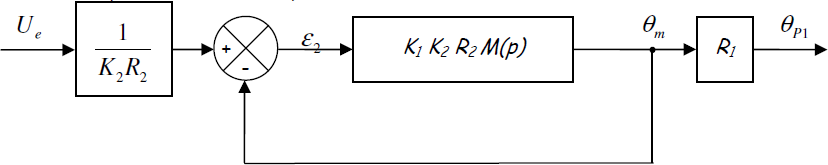
\includegraphics[width=.7\textwidth]{png/image4}
\end{center}

Le rapport de transmission du réducteur \textbf{1} est $R_1=\dfrac{1}{150}$.

\subsection{Détermination de la fonction de transfert en boucle ouverte}
\subparagraph{}
\textit{Déterminer la fonction de transfert $T(p)=\dfrac{\theta_{m}(p)}{\varepsilon_2(p)}$, la mettre sous la forme 
$T(p)=\dfrac{K_{BO}}{p\left( 1+\tau_m p\right)}$ et en déduire l'expression du gain de la boucle $K_{BO}$.}

\subsection{Détermination de la fonction de transfert en boucle fermée}
\subparagraph{}
\textit{Déterminer la fonction de transfert $F(p)=\dfrac{\theta_{P1}(p)}{U_e(p)}$ et montrer qu'elle peut se mettre sous la forme d'un système du second ordre. On notera $K_{BF}$ le gain statique $\xi$ le coefficient d'amortissement et $\omega_0$ la pulsation propre.}

\subparagraph{}
\textit{Donner l'expression littérale de $K_{BF}$ en fonction de $R_1$, $R_2$ et $K_2$ de $\xi$ et $\omega_0$ en fonction de $K_{BO}$ et $\tau_m$.}


\subsection{Analyse des performances}
\subparagraph{\label{ques}}
\textit{Déterminer la valeur du gain de boucle $K_{BO}$ de telle sorte que la réponse à une entrée de type échelon soit la plus rapide possible sans toutefois produire de dépassement.}

\subparagraph{}
\textit{Déterminer l'écart de position pour une entrée de type échelon en calculant l'écart statique : 
$\varepsilon_s = \lim\limits_{t\to +\infty}\varepsilon_2(t)$. Le système est précis à une entrée de type échelon si $\varepsilon_S=0$. Conclure.}

\subparagraph{}
\textit{Déterminer le temps de réponse à 5\% à l'aide de la figure 3.}


\begin{center}
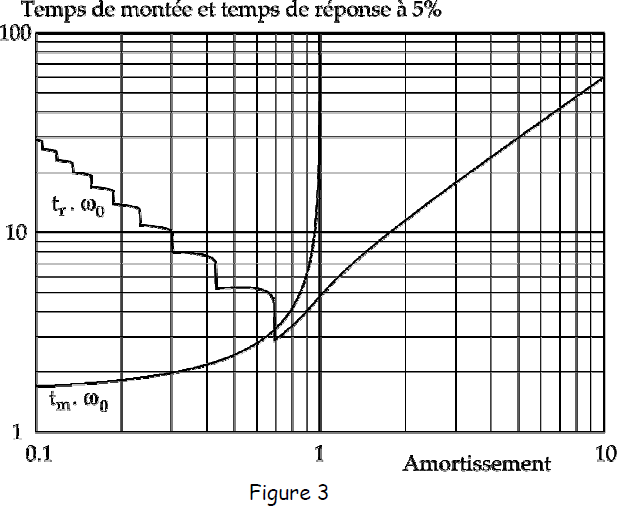
\includegraphics[width=.7\textwidth]{png/image5}
\end{center}



%\subsection{Détermination du gain $K_1$}
%On admet que la longueur utile de la vis est $l = 0,6\;m$. Le pas de la vis est $p_v=10\;mm$ (distance
%parcourue quand la vis à fait un tour).
%
%\subparagraph{}
%\textit{Déterminer le nombre de tour maximal $N_v$ que va faire la vis.}
%
%La vis est entraînée en rotation par un réducteur \textbf{52} dont le rapport de réduction est 
%$\dfrac{\theta_{P1}}{\theta_v}=\dfrac{1}{5}$.
%
%
%\subparagraph{}
%\textit{Déterminer le nombre de tour $N_{P1}$ que va faire l’arbre d’entrée du réducteur \textbf{52}.
%L’arbre d’entrée du réducteur \textbf{52} est entraîné par le réducteur \textbf{1}.}
%
%\subparagraph{}
%\textit{En déduire le nombre de tour $N_m$ que va faire l’arbre du moteur.}
%
%Le capteur de position de gain $K_2$ de la boucle d’asservissement du moteur électrique est un capteur
%potentiométrique 10 tours dont la tension de sortie varie de -12 à +12 Volts.
%
%\subparagraph{}
%\textit{En supposant que l’on utilise le capteur sur toute sa plage (10 tours), déterminer le rapport
%de réduction $R_2$ du réducteur reliant la sortie du moteur à l’entrée du potentiomètre.}
%
%\subparagraph{}
%\textit{Déterminer le gain du capteur potentiométrique.}
%
%\subparagraph{}
%\textit{En déduire le gain $K_1$ du régulateur connaissant la valeur de $K_{BO}$ fixée lors de la \textbf{Question \ref{ques}}.}

\subsection{Analyse des performances en mode suiveur}
Dans le cas d’une entrée de type rampe $u_e(t) = t u(t)$, le cahier des charges stipule que l’écart de
traînage ne doit pas excéder $\varepsilon_T \leq 0,5\;rad$.

\subparagraph{}
\textit{Déterminer l’écart de traînage $\varepsilon_T =\lim\limits_{t\to +\infty} \varepsilon_2(t)$ à une entrée de type rampe.}

\subparagraph{}
\textit{En déduire une première inégalité sur $K_{BO}$ permettant de vérifier cette partie du cahier
charges.}

\subparagraph{}
\textit{En reprenant la \textbf{Question \ref{ques}}, déterminer une seconde inégalité sur $K_{BO}$ permettant d’assurer que la réponse indicielle du système ne présentera pas de dépassement.}

Dans la pratique le régulateur est un correcteur dont la fonction de transfert est :
$$
C_1(p)=K_1\dfrac{1+T_1 p}{1+bT_1 p} \text{ avec } b>1
$$


\subparagraph{}
\textit{Justifier la nécessité de ce correcteur.}





\end{document}
